% Options for packages loaded elsewhere
\PassOptionsToPackage{unicode}{hyperref}
\PassOptionsToPackage{hyphens}{url}
\PassOptionsToPackage{dvipsnames,svgnames,x11names}{xcolor}
%
\documentclass[
  letterpaper,
  DIV=11,
  numbers=noendperiod]{scrartcl}

\usepackage{amsmath,amssymb}
\usepackage{iftex}
\ifPDFTeX
  \usepackage[T1]{fontenc}
  \usepackage[utf8]{inputenc}
  \usepackage{textcomp} % provide euro and other symbols
\else % if luatex or xetex
  \usepackage{unicode-math}
  \defaultfontfeatures{Scale=MatchLowercase}
  \defaultfontfeatures[\rmfamily]{Ligatures=TeX,Scale=1}
\fi
\usepackage{lmodern}
\ifPDFTeX\else  
    % xetex/luatex font selection
\fi
% Use upquote if available, for straight quotes in verbatim environments
\IfFileExists{upquote.sty}{\usepackage{upquote}}{}
\IfFileExists{microtype.sty}{% use microtype if available
  \usepackage[]{microtype}
  \UseMicrotypeSet[protrusion]{basicmath} % disable protrusion for tt fonts
}{}
\makeatletter
\@ifundefined{KOMAClassName}{% if non-KOMA class
  \IfFileExists{parskip.sty}{%
    \usepackage{parskip}
  }{% else
    \setlength{\parindent}{0pt}
    \setlength{\parskip}{6pt plus 2pt minus 1pt}}
}{% if KOMA class
  \KOMAoptions{parskip=half}}
\makeatother
\usepackage{xcolor}
\setlength{\emergencystretch}{3em} % prevent overfull lines
\setcounter{secnumdepth}{-\maxdimen} % remove section numbering
% Make \paragraph and \subparagraph free-standing
\ifx\paragraph\undefined\else
  \let\oldparagraph\paragraph
  \renewcommand{\paragraph}[1]{\oldparagraph{#1}\mbox{}}
\fi
\ifx\subparagraph\undefined\else
  \let\oldsubparagraph\subparagraph
  \renewcommand{\subparagraph}[1]{\oldsubparagraph{#1}\mbox{}}
\fi


\providecommand{\tightlist}{%
  \setlength{\itemsep}{0pt}\setlength{\parskip}{0pt}}\usepackage{longtable,booktabs,array}
\usepackage{calc} % for calculating minipage widths
% Correct order of tables after \paragraph or \subparagraph
\usepackage{etoolbox}
\makeatletter
\patchcmd\longtable{\par}{\if@noskipsec\mbox{}\fi\par}{}{}
\makeatother
% Allow footnotes in longtable head/foot
\IfFileExists{footnotehyper.sty}{\usepackage{footnotehyper}}{\usepackage{footnote}}
\makesavenoteenv{longtable}
\usepackage{graphicx}
\makeatletter
\def\maxwidth{\ifdim\Gin@nat@width>\linewidth\linewidth\else\Gin@nat@width\fi}
\def\maxheight{\ifdim\Gin@nat@height>\textheight\textheight\else\Gin@nat@height\fi}
\makeatother
% Scale images if necessary, so that they will not overflow the page
% margins by default, and it is still possible to overwrite the defaults
% using explicit options in \includegraphics[width, height, ...]{}
\setkeys{Gin}{width=\maxwidth,height=\maxheight,keepaspectratio}
% Set default figure placement to htbp
\makeatletter
\def\fps@figure{htbp}
\makeatother

\KOMAoption{captions}{tableheading}
\makeatletter
\@ifpackageloaded{caption}{}{\usepackage{caption}}
\AtBeginDocument{%
\ifdefined\contentsname
  \renewcommand*\contentsname{Table of contents}
\else
  \newcommand\contentsname{Table of contents}
\fi
\ifdefined\listfigurename
  \renewcommand*\listfigurename{List of Figures}
\else
  \newcommand\listfigurename{List of Figures}
\fi
\ifdefined\listtablename
  \renewcommand*\listtablename{List of Tables}
\else
  \newcommand\listtablename{List of Tables}
\fi
\ifdefined\figurename
  \renewcommand*\figurename{Figure}
\else
  \newcommand\figurename{Figure}
\fi
\ifdefined\tablename
  \renewcommand*\tablename{Table}
\else
  \newcommand\tablename{Table}
\fi
}
\@ifpackageloaded{float}{}{\usepackage{float}}
\floatstyle{ruled}
\@ifundefined{c@chapter}{\newfloat{codelisting}{h}{lop}}{\newfloat{codelisting}{h}{lop}[chapter]}
\floatname{codelisting}{Listing}
\newcommand*\listoflistings{\listof{codelisting}{List of Listings}}
\makeatother
\makeatletter
\makeatother
\makeatletter
\@ifpackageloaded{caption}{}{\usepackage{caption}}
\@ifpackageloaded{subcaption}{}{\usepackage{subcaption}}
\makeatother
\ifLuaTeX
  \usepackage{selnolig}  % disable illegal ligatures
\fi
\usepackage{bookmark}

\IfFileExists{xurl.sty}{\usepackage{xurl}}{} % add URL line breaks if available
\urlstyle{same} % disable monospaced font for URLs
\hypersetup{
  pdftitle={Slide Decks for John Curtin's Scientific Presentations},
  pdfauthor={John J. Curtin},
  colorlinks=true,
  linkcolor={blue},
  filecolor={Maroon},
  citecolor={Blue},
  urlcolor={Blue},
  pdfcreator={LaTeX via pandoc}}

\title{Slide Decks for John Curtin's Scientific Presentations}
\author{John J. Curtin}
\date{2024-03-14}

\begin{document}
\maketitle

\subsection{Overview}\label{overview}

\subsection{Generic}\label{generic}

\subsection{MATCH}\label{match}

\subsubsection{AIM 2}\label{aim-2}

A series of figures that add bars to unpack Aim 2 primary results

\begin{figure}[H]

\centering{

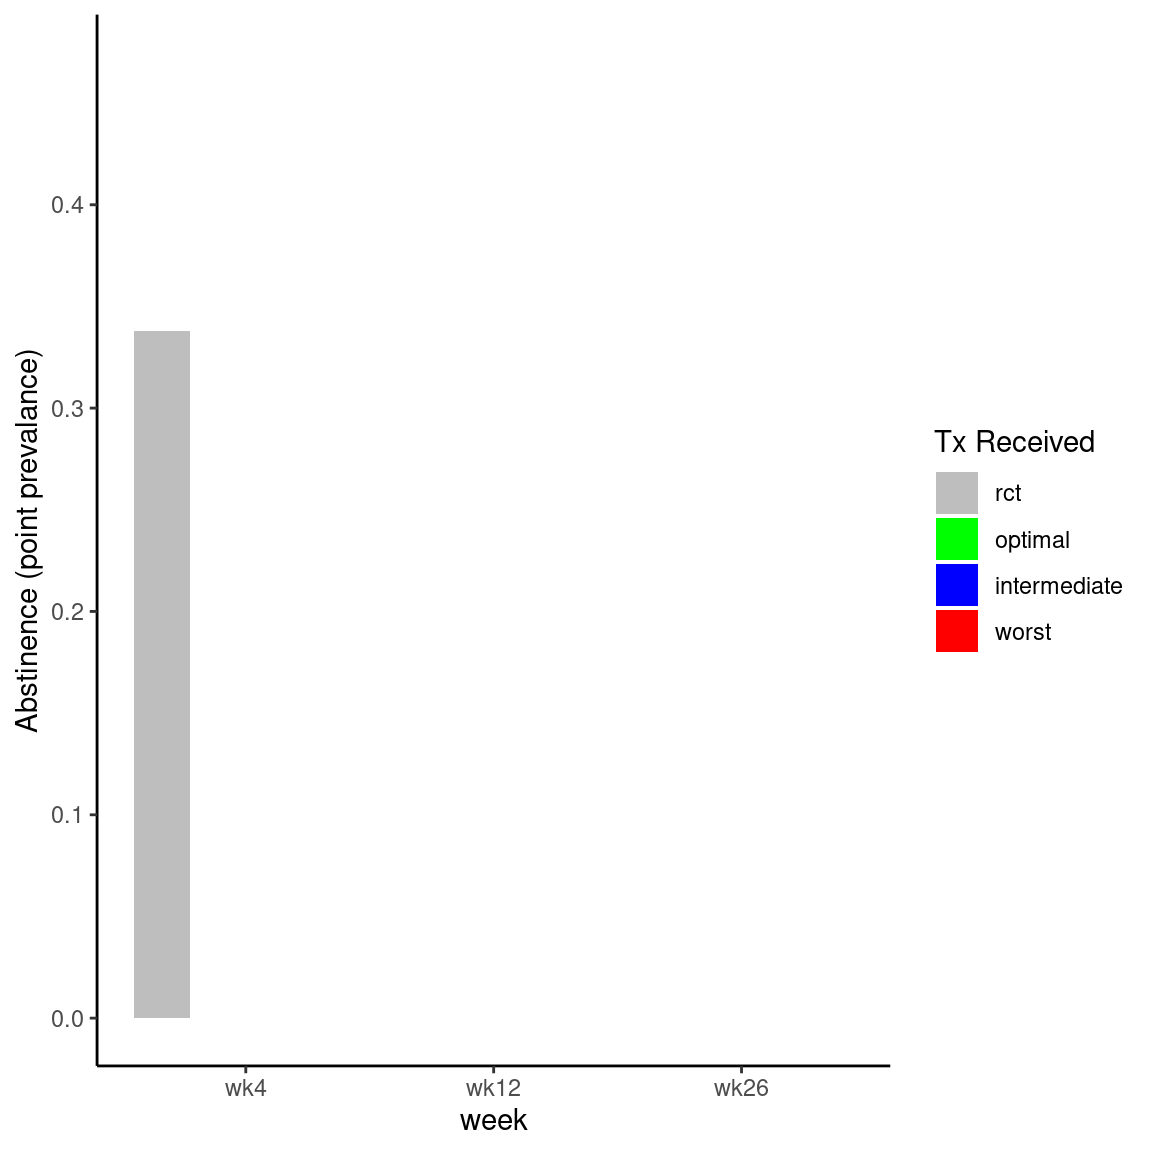
\includegraphics{index_files/figure-latex/notebooks-match_figs-fig-tx_week_1-output-1.png}

}

\caption{\label{fig-tx_week_1}Abstince Rate over Time by Tx Received}

\end{figure}%

\textsubscript{Source:
\href{https://jjcurtin.github.io/lectures_science/notebooks/match_figs-preview.html\#cell-fig-tx_week_1}{Match
Figures}}

\begin{figure}[H]

\centering{

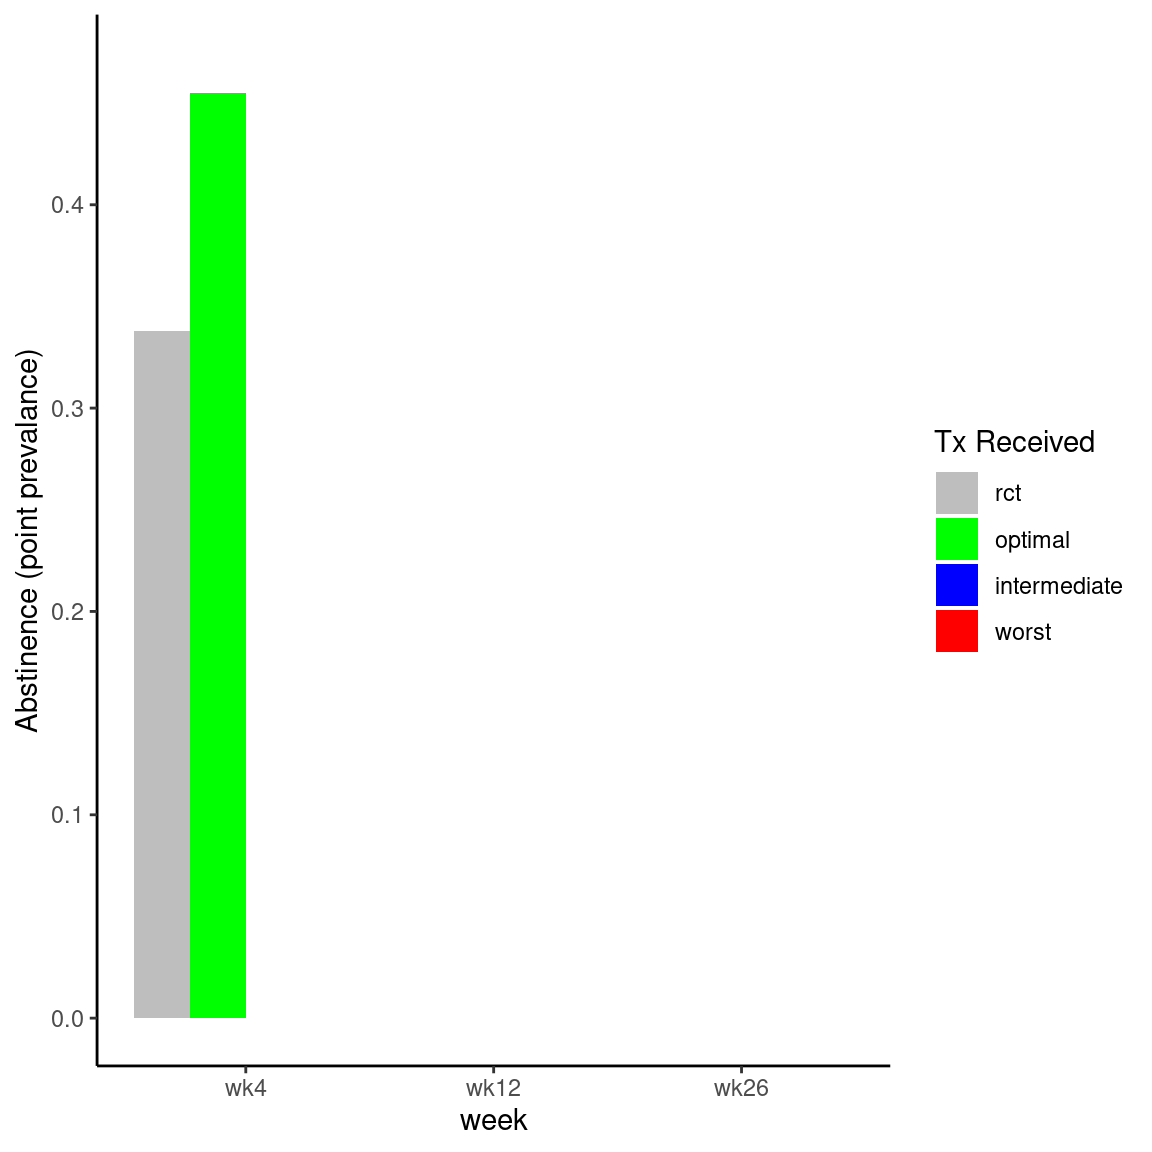
\includegraphics{index_files/figure-latex/notebooks-match_figs-fig-tx_week_2-output-1.png}

}

\caption{\label{fig-tx_week_2}Abstince Rate over Time by Tx Received}

\end{figure}%

\textsubscript{Source:
\href{https://jjcurtin.github.io/lectures_science/notebooks/match_figs-preview.html\#cell-fig-tx_week_2}{Match
Figures}}

\begin{figure}[H]

\centering{

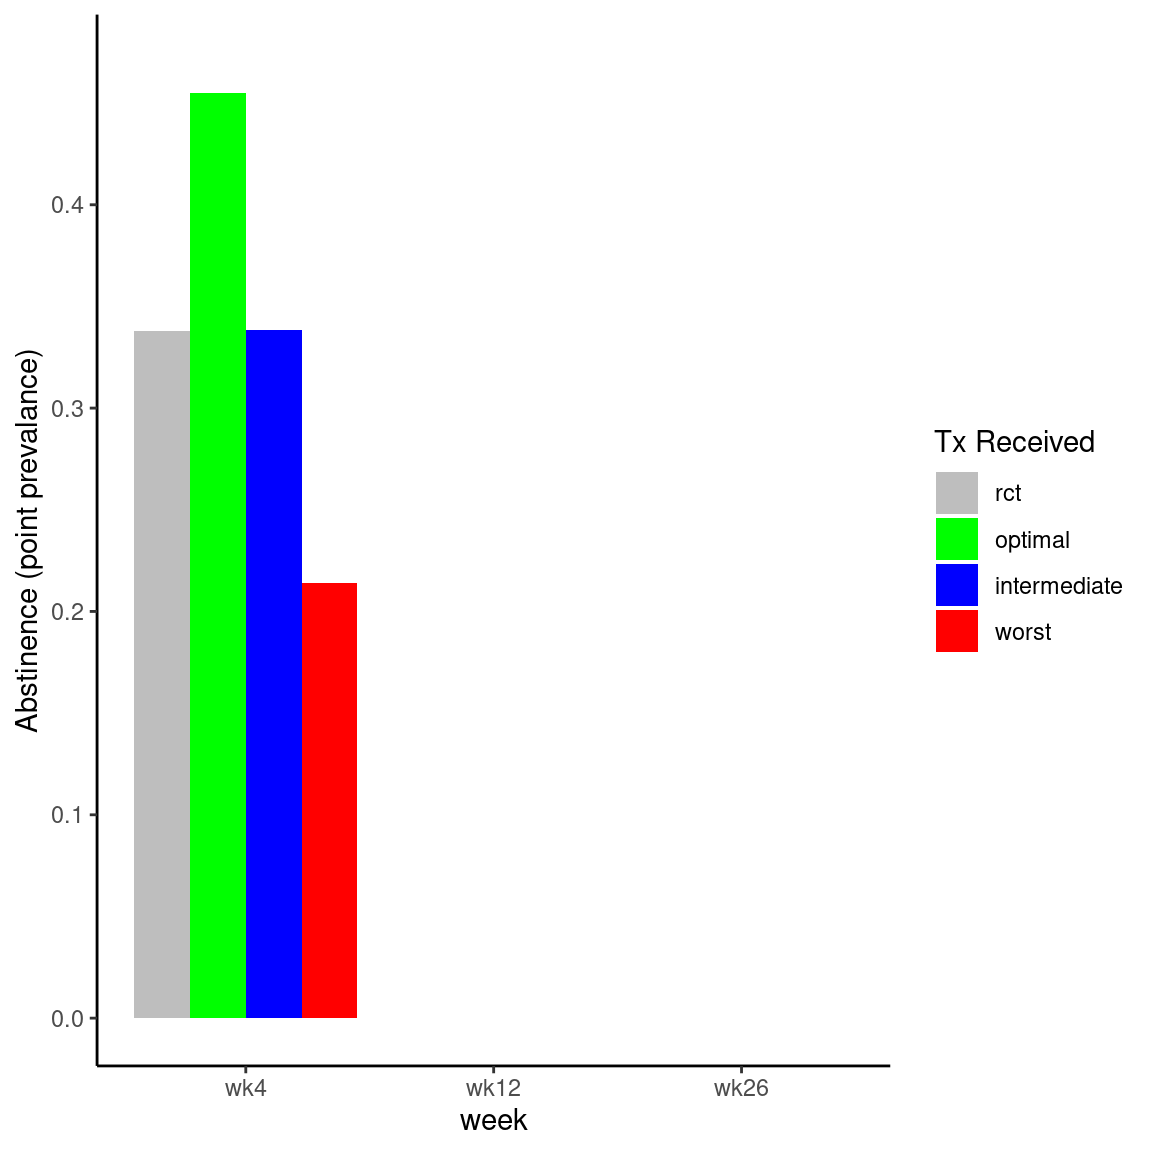
\includegraphics{index_files/figure-latex/notebooks-match_figs-fig-tx_week_3-output-1.png}

}

\caption{\label{fig-tx_week_3}Abstince Rate over Time by Tx Received}

\end{figure}%

\textsubscript{Source:
\href{https://jjcurtin.github.io/lectures_science/notebooks/match_figs-preview.html\#cell-fig-tx_week_3}{Match
Figures}}

\begin{figure}[H]

\centering{

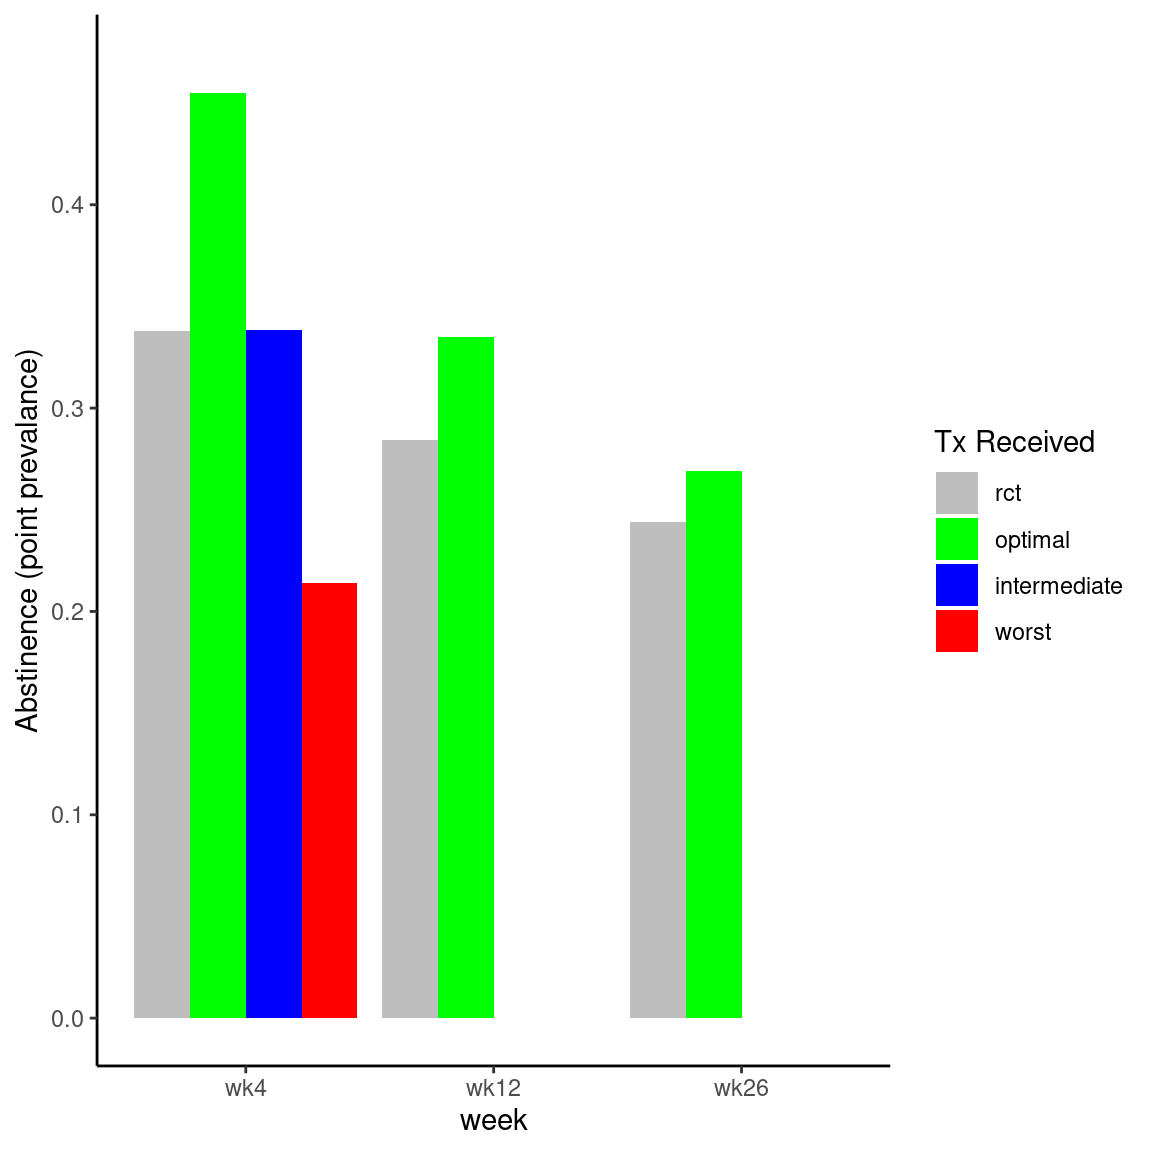
\includegraphics{index_files/figure-latex/notebooks-match_figs-fig-tx_week_4-output-1.png}

}

\caption{\label{fig-tx_week_4}Abstince Rate over Time by Tx Received}

\end{figure}%

\textsubscript{Source:
\href{https://jjcurtin.github.io/lectures_science/notebooks/match_figs-preview.html\#cell-fig-tx_week_4}{Match
Figures}}

\begin{figure}[H]

\centering{

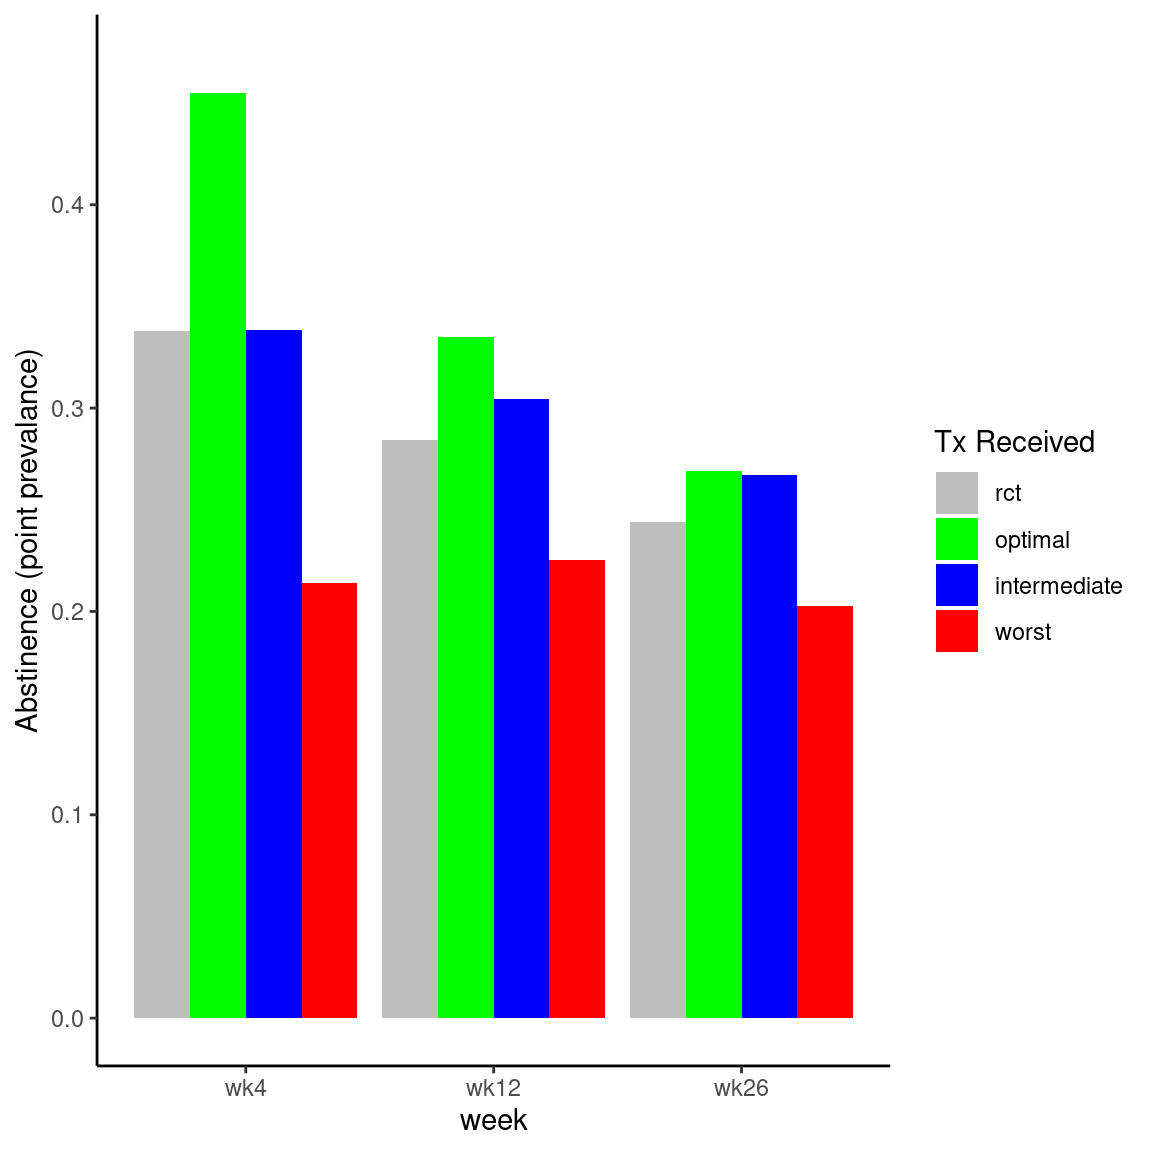
\includegraphics{index_files/figure-latex/notebooks-match_figs-fig-tx_week_5-output-1.png}

}

\caption{\label{fig-tx_week_5}Abstince Rate over Time by Tx Received}

\end{figure}%

\textsubscript{Source:
\href{https://jjcurtin.github.io/lectures_science/notebooks/match_figs-preview.html\#cell-fig-tx_week_5}{Match
Figures}}

\subsection{Burden Study}\label{burden-study}

\subsection{EMA Study}\label{ema-study}

\subsubsection{Probability Histograms}\label{probability-histograms}

\begin{figure}[H]

\centering{

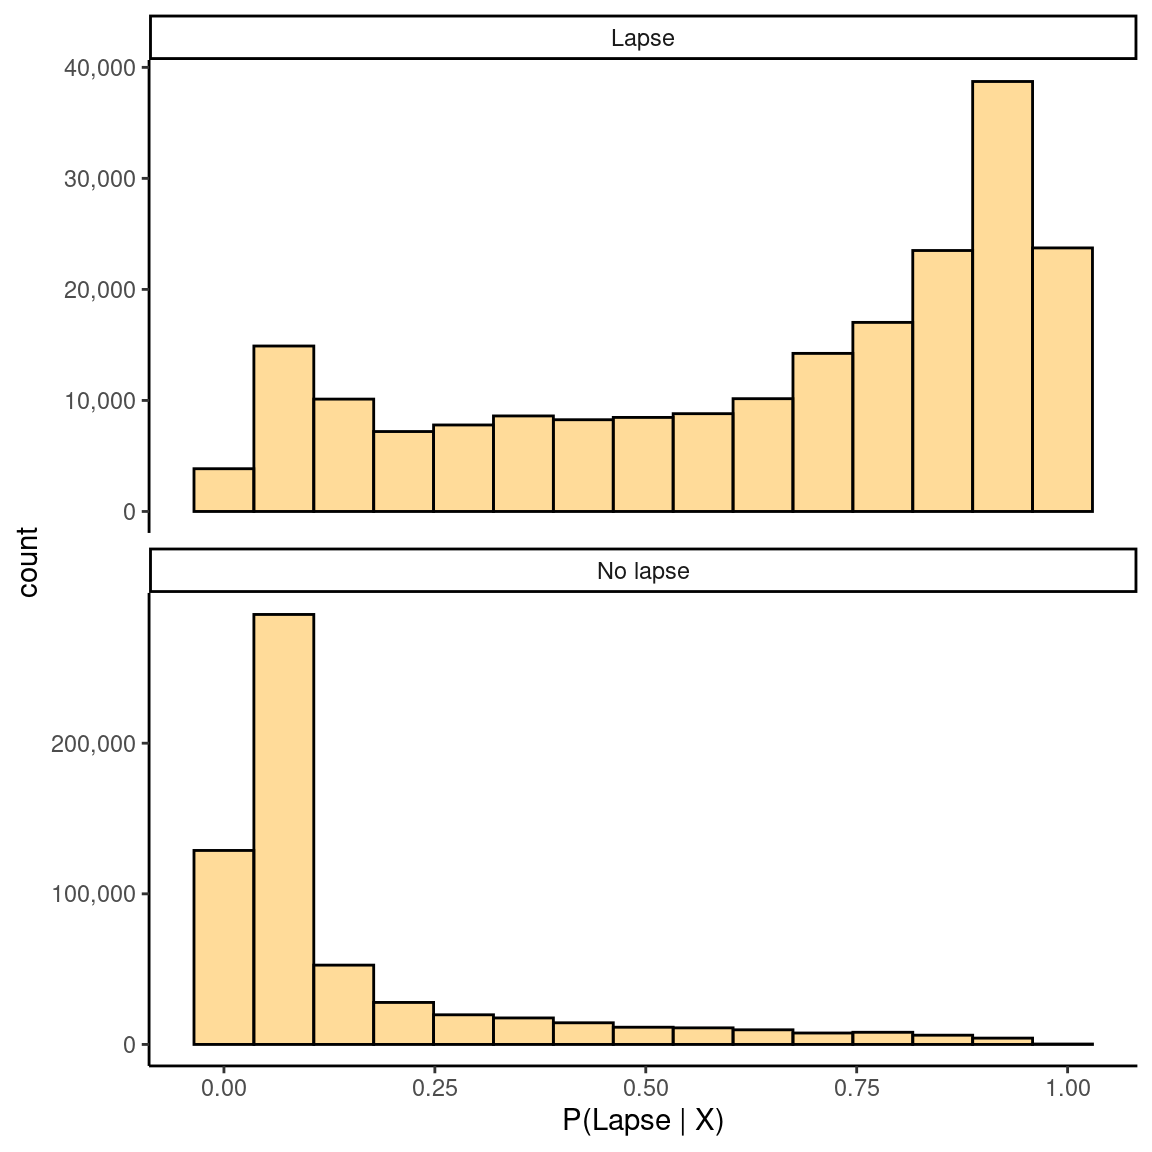
\includegraphics{index_files/figure-latex/notebooks-ema_figs_probability-fig-week-no_dec_thres-output-1.png}

}

\caption{\label{fig-week-no_dec_thres}P(Lapse \textbar{} X) by Truth -
Week}

\end{figure}%

\textsubscript{Source:
\href{https://jjcurtin.github.io/lectures_science/notebooks/ema_figs_probability-preview.html\#cell-fig-week-no_dec_thres}{Risk1
probability plots}}

\begin{figure}[H]

\centering{

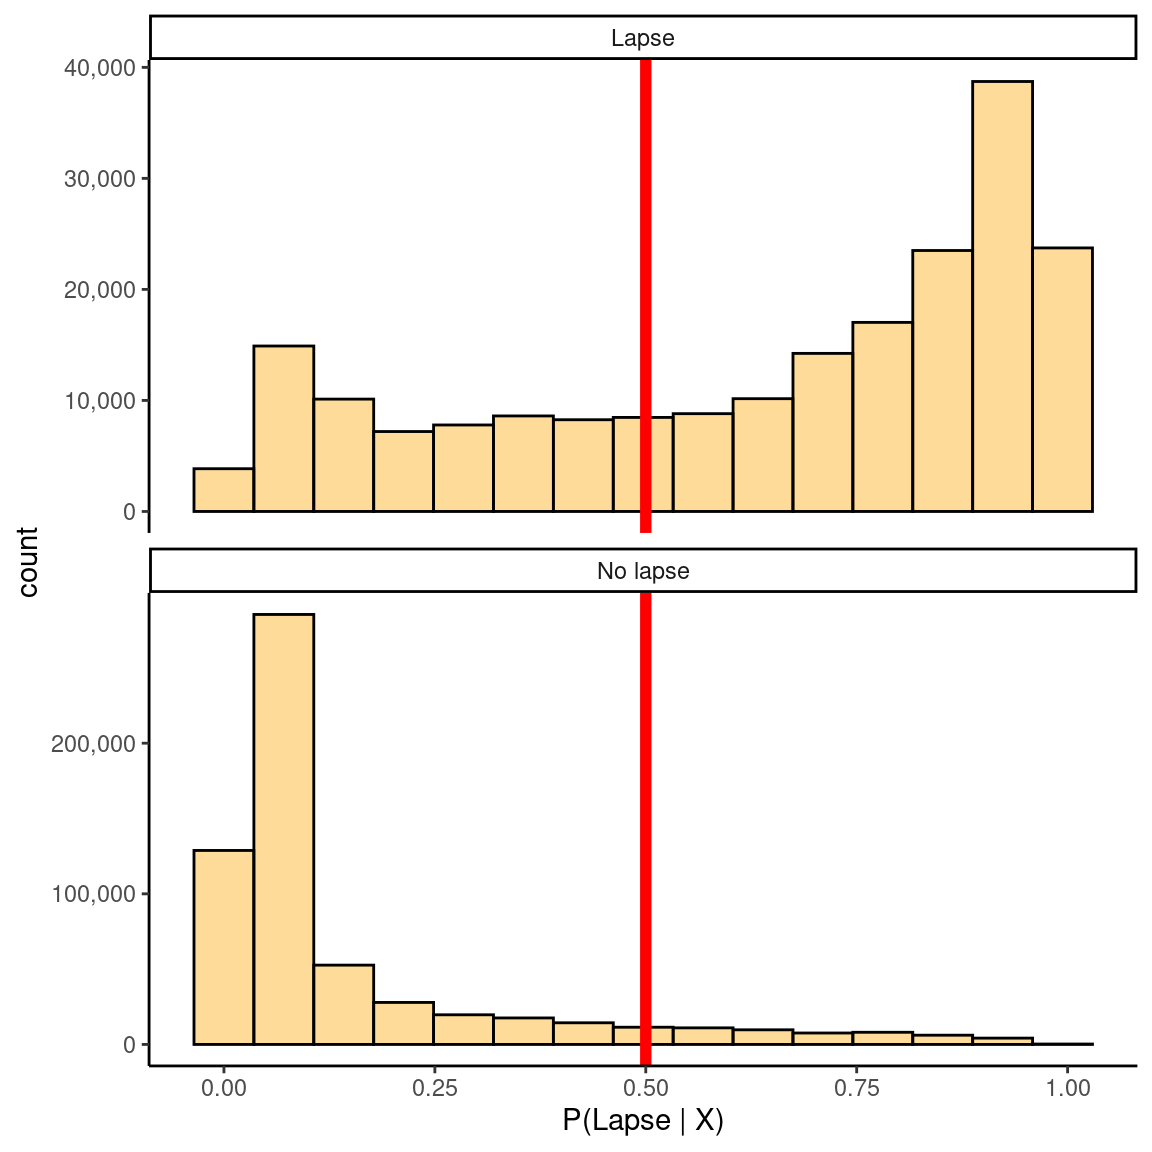
\includegraphics{index_files/figure-latex/notebooks-ema_figs_probability-fig-week-output-2.png}

}

\caption{\label{fig-week}P(Lapse \textbar{} X) by Truth - Day}

\end{figure}%

\textsubscript{Source:
\href{https://jjcurtin.github.io/lectures_science/notebooks/ema_figs_probability-preview.html\#cell-fig-week}{Risk1
probability plots}}

\begin{figure}[H]

\centering{

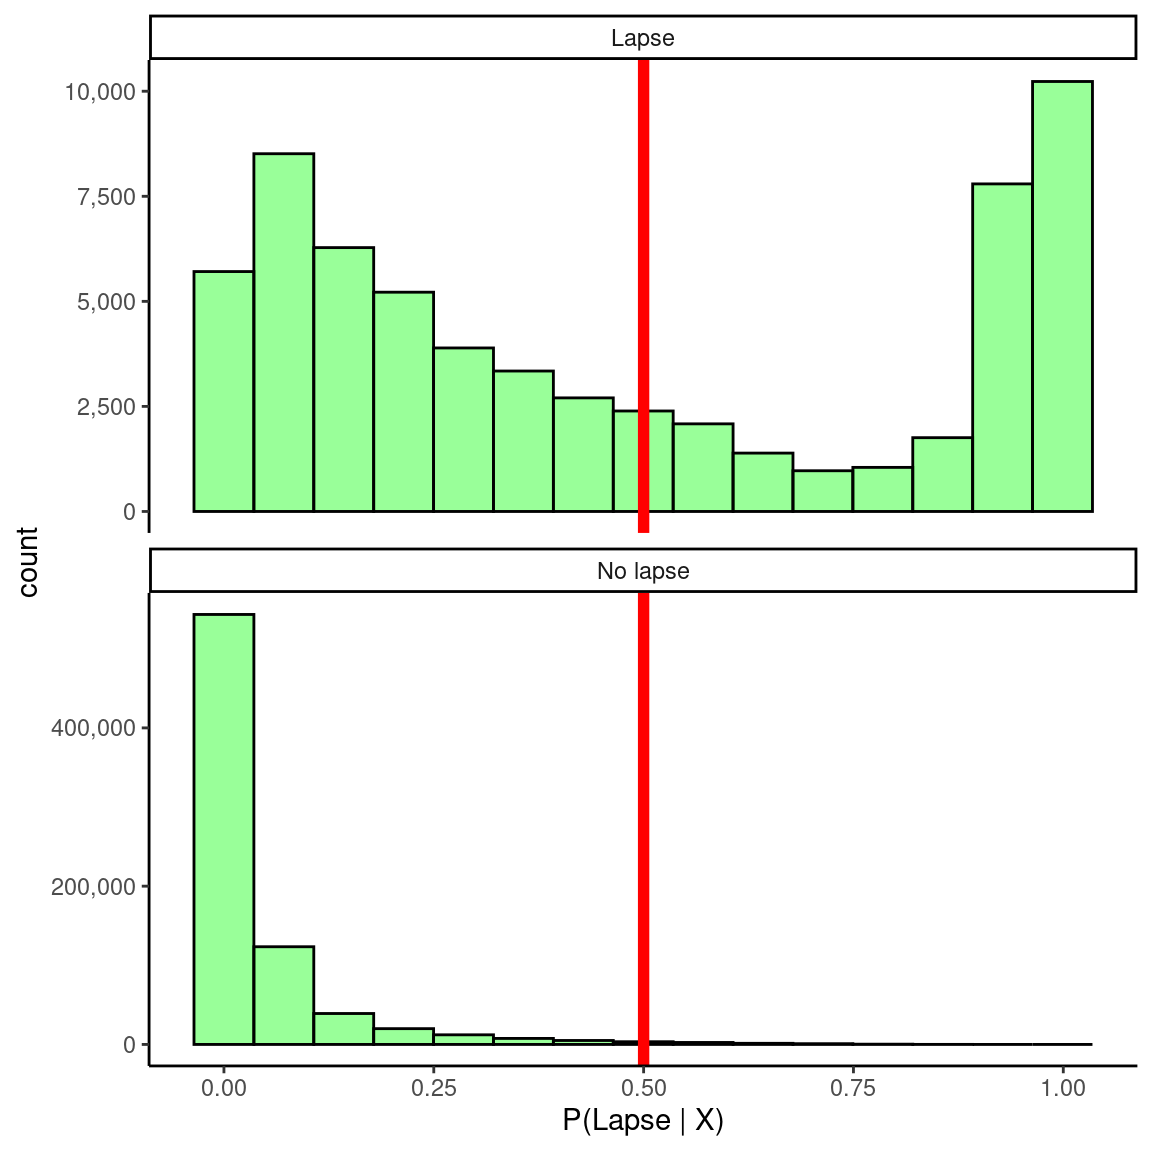
\includegraphics{index_files/figure-latex/notebooks-ema_figs_probability-fig-day-output-1.png}

}

\caption{\label{fig-day}P(Lapse \textbar{} X) by Truth - Hour}

\end{figure}%

\textsubscript{Source:
\href{https://jjcurtin.github.io/lectures_science/notebooks/ema_figs_probability-preview.html\#cell-fig-day}{Risk1
probability plots}}

\begin{figure}[H]

\centering{

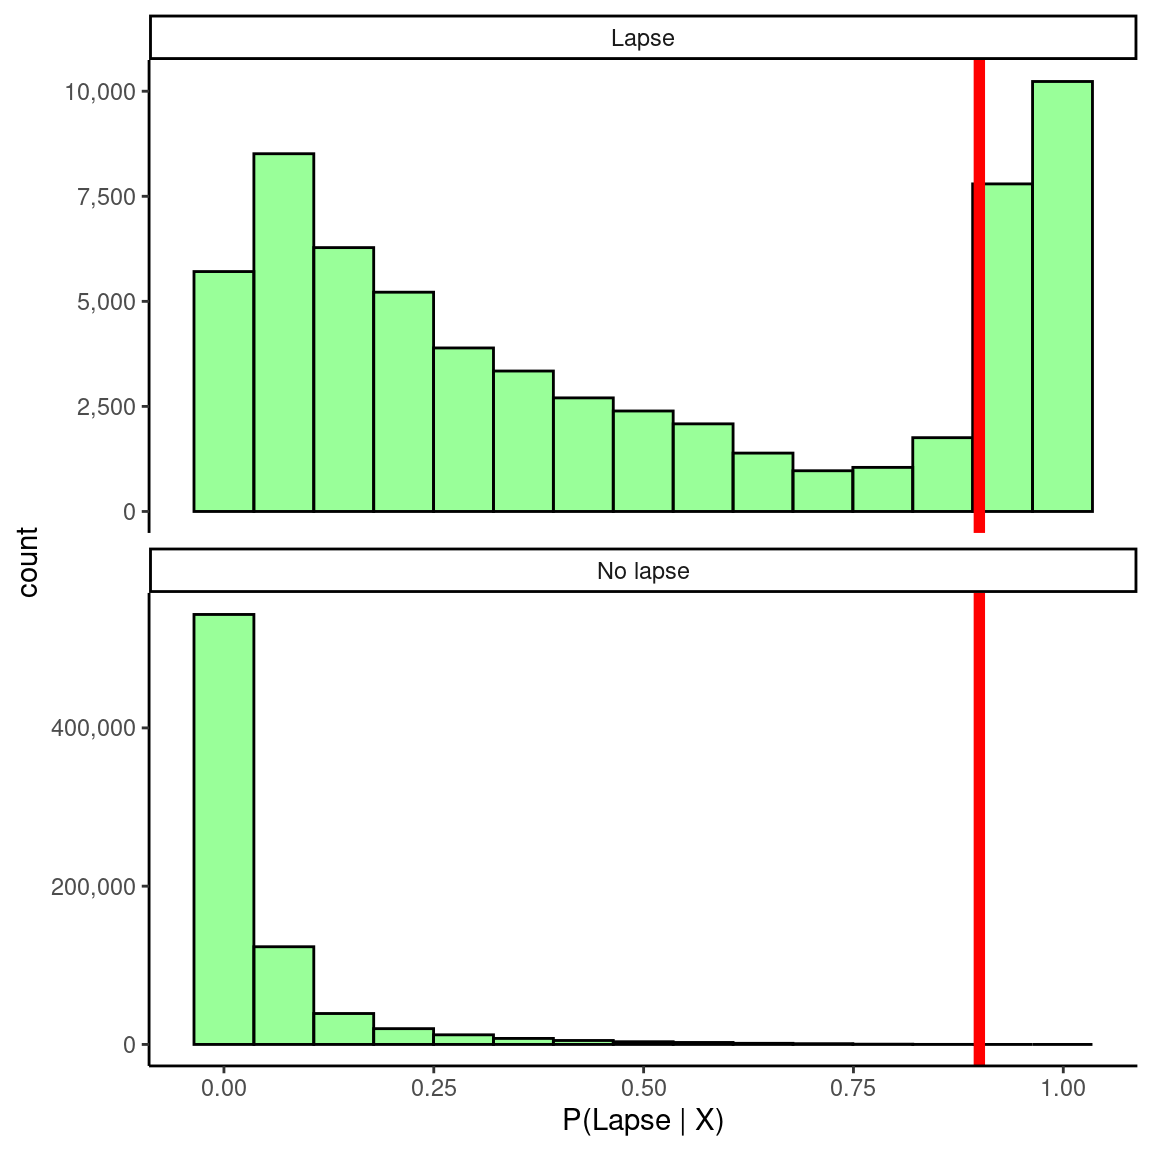
\includegraphics{index_files/figure-latex/notebooks-ema_figs_probability-fig-day-high_dec_thres-output-1.png}

}

\caption{\label{fig-day-high_dec_thres}Lapse Probability by Truth - Day}

\end{figure}%

\textsubscript{Source:
\href{https://jjcurtin.github.io/lectures_science/notebooks/ema_figs_probability-preview.html\#cell-fig-day-high_dec_thres}{Risk1
probability plots}}

\subsubsection{ROCs}\label{rocs}

\begin{figure}[H]

\centering{

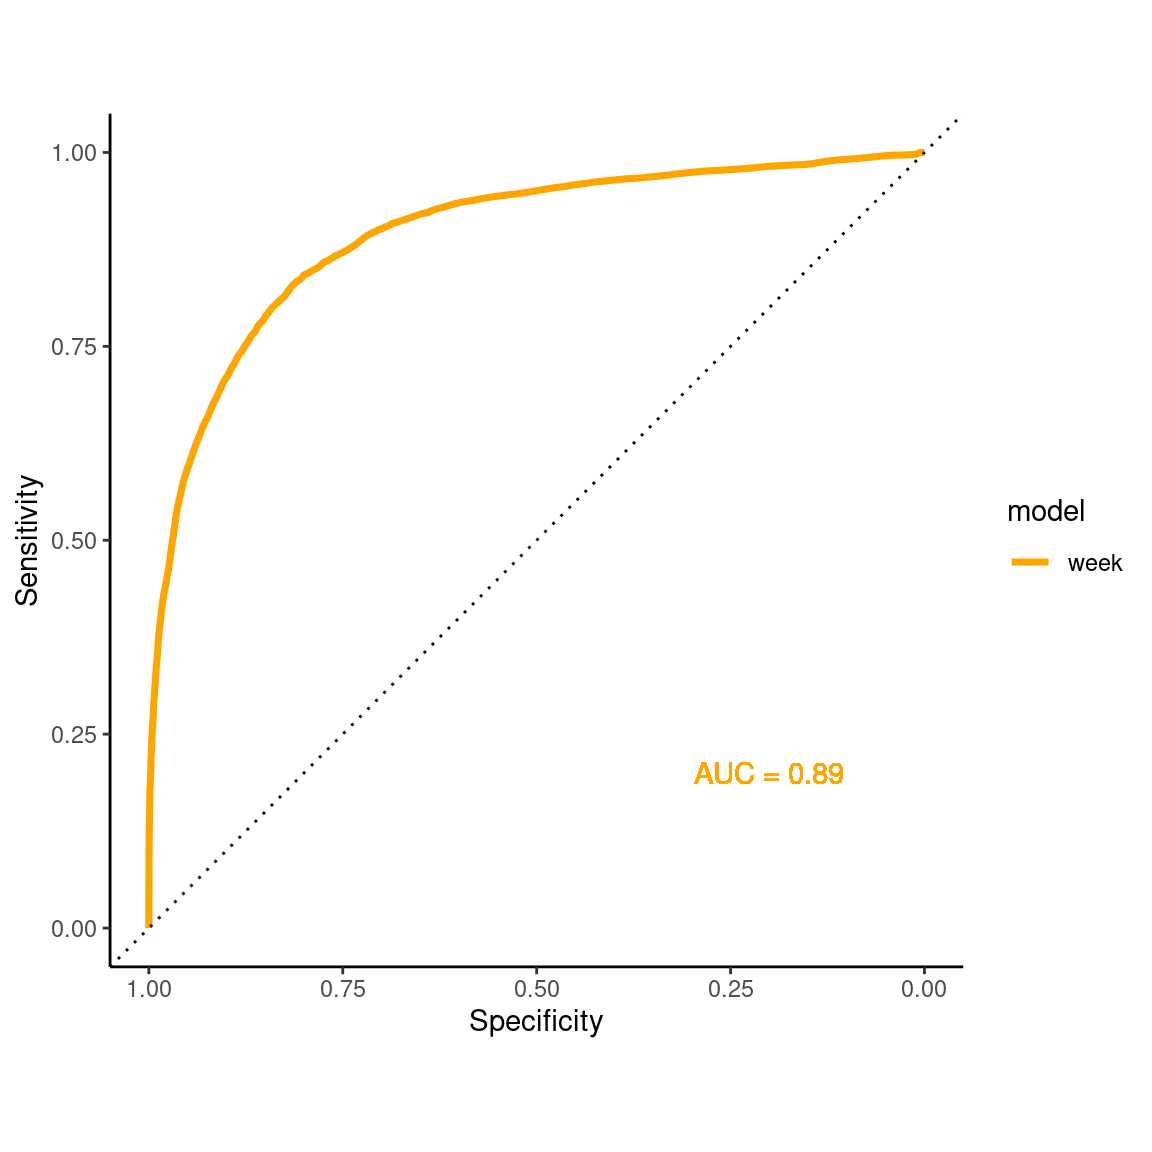
\includegraphics{index_files/figure-latex/notebooks-ema_figs_roc-fig-roc-week-output-1.png}

}

\caption{\label{fig-roc-week}ROC Curves by Model}

\end{figure}%

\textsubscript{Source:
\href{https://jjcurtin.github.io/lectures_science/notebooks/ema_figs_roc-preview.html\#cell-fig-roc-week}{EMA
ROCs}}

\begin{figure}[H]

\centering{

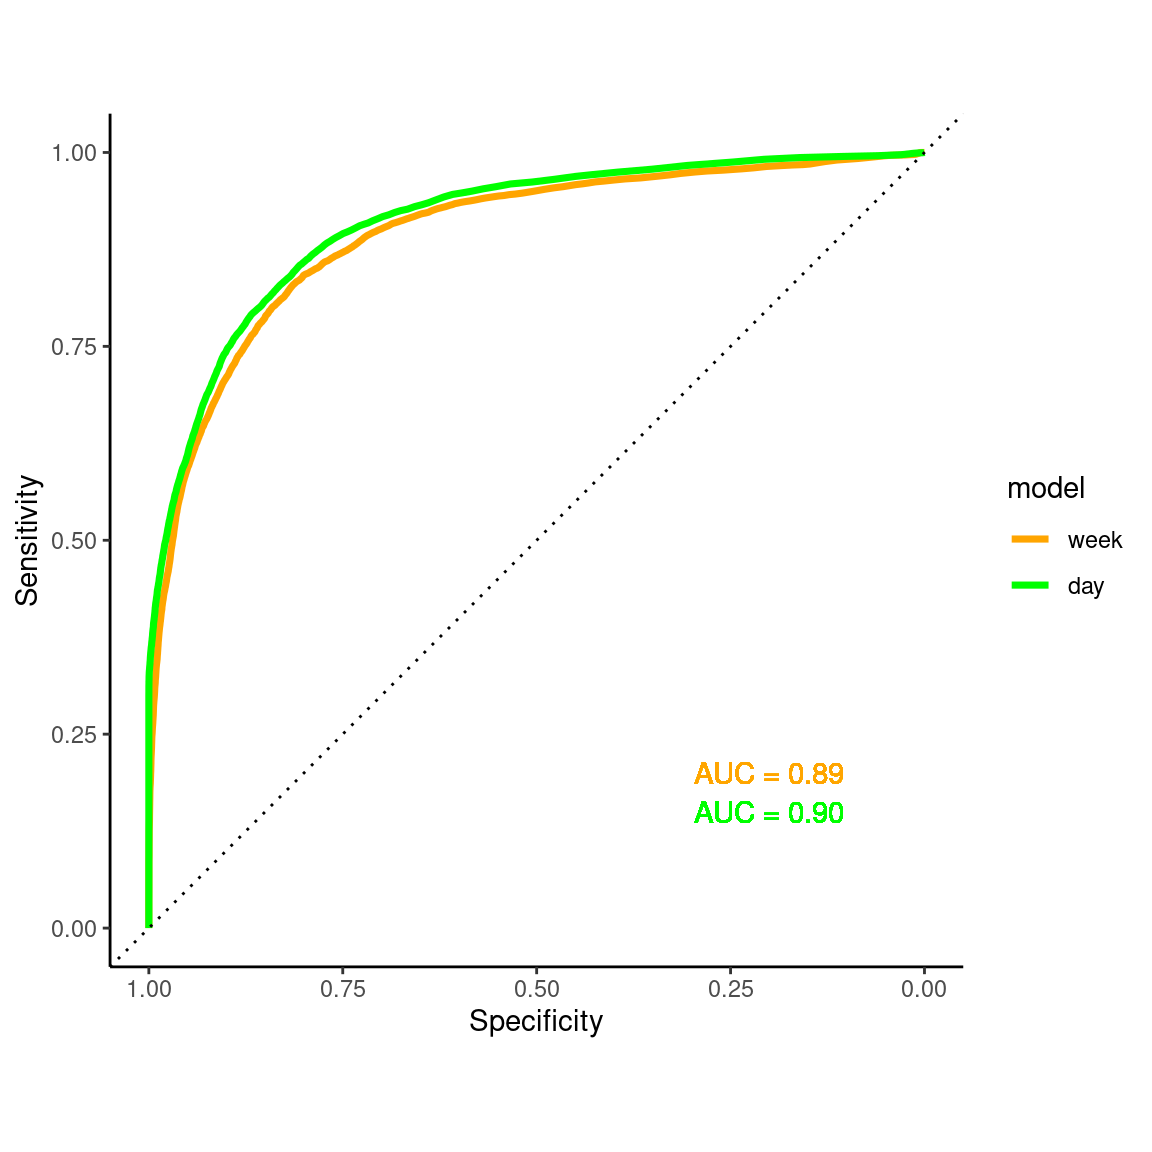
\includegraphics{index_files/figure-latex/notebooks-ema_figs_roc-fig-roc-week_day-output-1.png}

}

\caption{\label{fig-roc-week_day}ROC Curves by Model}

\end{figure}%

\textsubscript{Source:
\href{https://jjcurtin.github.io/lectures_science/notebooks/ema_figs_roc-preview.html\#cell-fig-roc-week_day}{EMA
ROCs}}

\begin{figure}[H]

\centering{

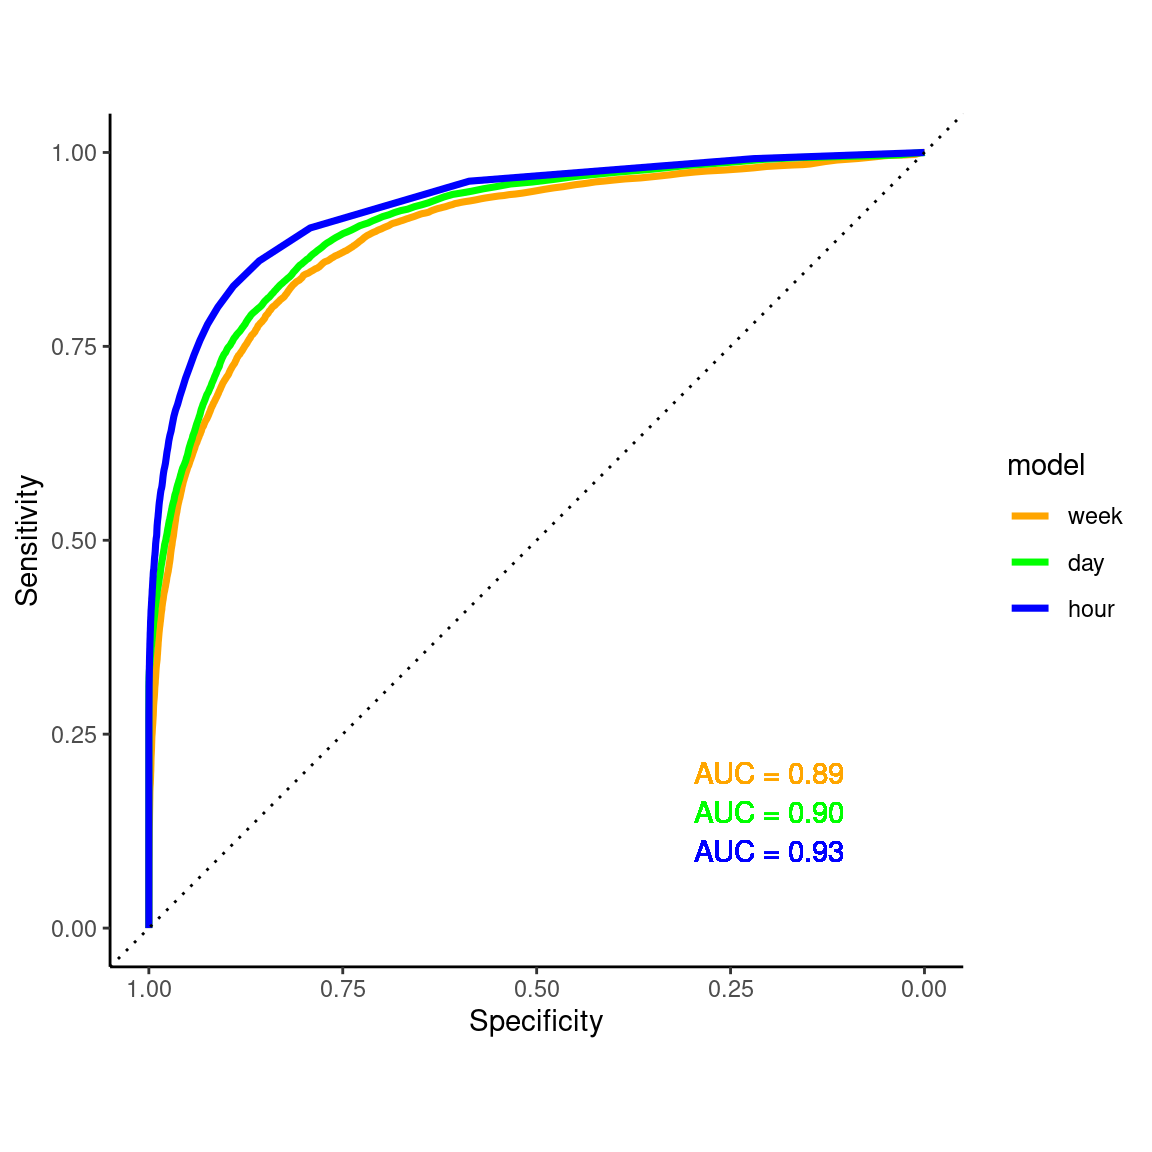
\includegraphics{index_files/figure-latex/notebooks-ema_figs_roc-fig-roc-all-output-1.png}

}

\caption{\label{fig-roc-all}ROC Curves by Model}

\end{figure}%

\textsubscript{Source:
\href{https://jjcurtin.github.io/lectures_science/notebooks/ema_figs_roc-preview.html\#cell-fig-roc-all}{EMA
ROCs}}



\end{document}
